% This is samplepaper.tex, a sample chapter demonstrating the
% LLNCS macro package for Springer Computer Science proceedings;
% Version 2.20 of 2017/10/04
%
\documentclass[12pt,a4paper,roman]{article}
%
\usepackage{amsmath}
\usepackage{amssymb}
\usepackage{booktabs} % For pretty tables
\usepackage{caption} % For caption spacing
\usepackage{subcaption} % For sub-figures
\usepackage{graphicx}
\graphicspath{ {./figures/} }
\usepackage{pgfplots}
\usepackage[all]{nowidow}
\usepackage[utf8]{inputenc}
\usepackage{xcolor}
\usepackage{tikz}
\usepackage{tikz-feynman} 
\tikzfeynmanset{compat=1.0.0}
\usetikzlibrary{er,positioning,bayesnet}
\usepackage{multicol}
\usepackage{algpseudocode,algorithm,algorithmicx}
\usepackage{hyperref}
\usepackage[inline]{enumitem} % Horizontal lists
% Used for displaying a sample figure. If possible, figure files should
% be included in EPS format.
%
% If you use the hyperref package, please uncomment the following line
% to display URLs in blue roman font according to Springer's eBook style:
% \renewcommand\UrlFont{\color{blue}\rmfamily}

\newcommand{\card}[1]{\left\vert{#1}\right\vert}
\newcommand*\Let[2]{\State #1 $\gets$ #2}
\definecolor{blue}{HTML}{1F77B4}
\definecolor{orange}{HTML}{FF7F0E}
\definecolor{green}{HTML}{2CA02C}

\pgfplotsset{compat=1.14}

\renewcommand{\topfraction}{0.85}
\renewcommand{\bottomfraction}{0.85}
\renewcommand{\textfraction}{0.15}
\renewcommand{\floatpagefraction}{0.8}
\renewcommand{\textfraction}{0.1}
\setlength{\floatsep}{3pt plus 1pt minus 1pt}
\setlength{\textfloatsep}{3pt plus 1pt minus 1pt}
\setlength{\intextsep}{3pt plus 1pt minus 1pt}
\setlength{\abovecaptionskip}{2pt plus 1pt minus 1pt}

\begin{document}
%
\title{Formulaic collection for Keldysh mfRG calculations}
%
%\titlerunning{Abbreviated paper title}
% If the paper title is too long for the running head, you can set
% an abbreviated paper title here
%
\author{Santiago Aguirre \& Elias Walter}
%
%\authorrunning{F. Author et al.}
% First names are abbreviated in the running head.
% If there are more than two authors, 'et al.' is used.
%
%\institute{Ludwig-Maximilians University, Munich, Germany \\
%\email{\{sa.aguirre, e.walter\}@physik.uni-muenchen.de}}
%
\maketitle              % typeset the header of the contribution
%
% \begin{abstract}
% The efficiency of a query execution plan depends on the accuracy of the selectivity estimates given to the query optimiser by the cost model. The cost model makes simplifying assumptions in order to produce said estimates in a timely manner. These assumptions lead to selectivity estimation errors that have dramatic effects on the quality of the resulting query execution plans. A convenient assumption that is ubiquitous among current cost models is to assume that attributes are independent with each other. However, it ignores potential correlations which can have a huge negative impact on the accuracy of the cost model. In this paper we attempt to relax the attribute value independence assumption without unreasonably deteriorating the accuracy of the cost model. We propose a novel approach based on a particular type of Bayesian networks called Chow-Liu trees to approximate the distribution of attribute values inside each relation of a database. Our results on the TPC-DS benchmark show that our method is an order of magnitude more precise than other approaches whilst remaining reasonably efficient in terms of time and space.

% \keywords{Query optimisation \and Cost Model \and Selectivity Estimation \and Bayesian networks.}
% \end{abstract}
%
%
%
\section*{General properties of the four-point vertex}

\begin{equation}
    \Gamma = \Gamma_{1'2'|12} = \Gamma_{\sigma_1'\sigma_2'|\sigma_1\sigma_2}^{\alpha_1'\alpha_2'|\alpha_1\alpha_2}(q_1'q_2'|q_1q_2, \nu_1'\nu_2'|\nu_1\nu_2)
\end{equation}
\begin{figure}[H]
\centering
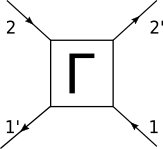
\includegraphics[scale=0.65]{vertex.png}
\caption{Convention for the vertex}
\label{fig:vertex}
\end{figure}
The Keldysh indices take values in the set $\{1,2\}$, with the convention $1 = q$ and $2=c$, where in some texts $c$ stands for 'classical component' and $q$ for 'quantum component'.
\subsection*{Spin conservation:}
Spin conservation: $\sigma_{1'} + \sigma_{2'} = \sigma_1 + \sigma_2$
Overall spin conservation of the vertex dictates that there are three (fundamentally, actually only two) different cases:
\subsubsection*{All spins equal}
Sum of the incoming (or outgoing) spins equals either -1 or 1: 
$\Gamma = \Gamma_{\sigma\sigma|\sigma\sigma}$
\subsubsection*{Incoming spins reversed}
Sum of incoming spins equals 0: 
$\Gamma = \Gamma_{\sigma\overline{\sigma}|\sigma\overline{\sigma}}$ or $\Gamma = \Gamma_{\sigma\overline{\sigma}|\overline{\sigma}\sigma}$
These last two cases can be linked through a spin-inversion transformation and, hence, aren't considered to be (computationally) different, although they represent distinct physical processes.

\subsection*{Frequency conservation:}
Conservation of momentum implies that one of the frequencies, conventionally chosen to be $\nu_2$, will be dependent on the other 3.
\begin{align}
    \nu_{1'} + \nu_{2'} &= \nu_1 + \nu_2  \\
    \implies \nu_2 &= \nu_{1'} + \nu_{2'} -\nu_1
\end{align}
Hence, we will omit $\nu_{2}$ altogether from all formulas it would have appeared in.

\subsection*{Causality:}
Causality, in the Keldysh formalism, translates to $\Gamma^{22|22} = 0$ always.

\subsection*{Particle exchange and complex conjugation:}
Here is how the vertex components are related under particle exchange:
\begin{align}
&\Gamma_{\sigma_2'\sigma_1'|\sigma_1\sigma_2}^{\alpha_2'\alpha_1'|\alpha_1\alpha_2}(q_2'q_1'|q_1q_2, \nu_2'\nu_1'|\nu_1\nu_2) \\
&= \Gamma_{\sigma_1'\sigma_2'|\sigma_2\sigma_1}^{\alpha_1'\alpha_2'|\alpha_2\alpha_1}(q_1'q_2'|q_2q_1, \nu_1'\nu_2'|\nu_2\nu_1) \\
&= - \Gamma_{\sigma_2'\sigma_1'|\sigma_2\sigma_1}^{\alpha_2'\alpha_1'|\alpha_2\alpha_1}(q_2'q_1'|q_2q_1, \nu_2'\nu_1'|\nu_2\nu_1) \\
&= - \Gamma_{\sigma_1'\sigma_2'|\sigma_1\sigma_2}^{\alpha_1'\alpha_2'|\alpha_1\alpha_2}(q_1'q_2'|q_1q_2, \nu_1'\nu_2'|\nu_1\nu_2)
\end{align}
And under complex conjugation:
\begin{multline}
\left[ \Gamma_{\sigma_1'\sigma_2'|\sigma_1\sigma_2}^{\alpha_1'\alpha_2'|\alpha_1\alpha_2}(q_1'q_2'|q_1q_2, \nu_1'\nu_2'|\nu_1\nu_2) \right]^* \\ =
(-1)^{(1+\alpha_1'+\alpha_2'+\alpha_1+\alpha_2)} \Gamma_{\sigma_1\sigma_2|\sigma_1'\sigma_2'}^{\alpha_1\alpha_2|\alpha_1'\alpha_2'}(q_1q_2|q_1'q_2', \nu_1\nu_2|\nu_1'\nu_2')
\end{multline}

\subsection*{Channel decomposition \& reducibility}
In the mfRG formalism we have that the full vertex can be written as the sum of the irreducible part $R = U + \mathcal{O}(u^4)$ and reducible contributions $\gamma_r$ in three channels: $r=a$ for \textit{anti-parallel}, $r=p$ for \textit{parallel} and $r=t$ for \textit{transverse}. These names allude to the relation of the cut propagator lines have, were one to make a diagram disconnected. Since any reducible diagram can only belong to one of these classes\cite{}, one can then write the following equation for the full vertex:
\begin{equation}
	\Gamma = R + \sum_r \gamma_r = R + \gamma_a + \gamma_p + \gamma_t
\end{equation}
This reducibility of the diagrams then gives rise to the ``bubble'' objects, $\Pi_r$, which are the pair of propagators that, should they be cut, would disconnect the diagram. These pairs of propagators effectively carry a (bosonic) transfer frequency between the two sides of the bubble. Knowing this, we can tailor an explicit frequency dependence that highlights and exploits this fact, in order to then simplify calculations. Hence, we introduce the following structures:

\begin{figure}[ht]
    \centering
    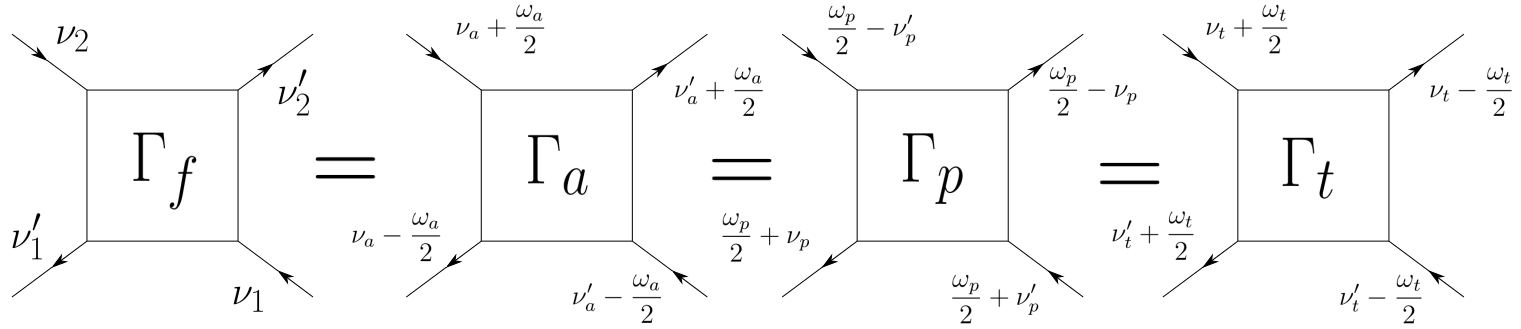
\includegraphics[width=\linewidth]{figures/channels_with_labels.png}
    \caption{Convention for the introduction of channel-specific frequencies}
    \label{fig:channels}
\end{figure}
In this notation we explicitly describe the full vertex function $\Gamma$, which is naturally a function of three arguments, as slight variations that depend on the convention for the respective channel. This means that all $\Gamma_r$ represent the same object, namely the full vertex, but each instantiation receives the arguments $\omega_r$, $\nu_r$ and $\nu'_r$, the bosonic and the two fermionic frequencies, respectively, already expressed in the channel's natural parametrization. This clarification is important since these objects are fundamentally different form the notationally-similar $\gamma_r$, which are the reducible vertices in the $r$-channel.

The frequencies in Fig. \ref{fig:channels} lead then to the following conversion rules between the channels, where the conventional vertex depicted in Fig. \ref{fig:vertex} is referred to as the 'fermionic' vertex, $\Gamma_f$:

\subsubsection*{a-channel}
From and to the fermionic channel:
\begin{align}
    \left.\begin{array}{r@{\mskip\thickmuskip}l}
    \nu_{1'} &= \nu_a - \frac{\omega_a}{2} \\
    \nu_{2'} &= \nu'_a + \frac{\omega_a}{2} \\
    \nu_{1 } &= \nu'_a - \frac{\omega_a}{2} \\
  \end{array} \right\}
  \quad \implies \quad
  \left\{\begin{array}{l@{\mskip\thickmuskip}l}
    \omega_a &= \nu_{2} - \nu_{1'} = \nu_{2'} - \nu_{1}\\
    \nu_a    &= \frac{1}{2}\left(2\nu_{1'}+\nu_{2'}-\nu_{1}\right) \\
    \nu'_a   &= \frac{1}{2}\left(\nu_{2'} + \nu_{1}\right)\\
  \end{array}\right.
\end{align}

And from any other channel to the a-channel:
\begin{align}
    \begin{array}{r@{\mskip\thickmuskip}l}
    \omega_a &= \omega_a\\
    \nu_a  &= \nu_a \\
    \nu'_a &= \nu'_a\\
  \end{array}
  \quad  \begin{array}{r@{\mskip\thickmuskip}l}
    \omega_a &= -\nu_p-\nu'_p\\
    \nu_a  &= \frac{\omega_p+\nu_p-\nu'_p}{2}\\
    \nu'_a &= \frac{\omega_p-\nu_p+\nu'_p}{2}\\
  \end{array} \quad
  \begin{array}{r@{\mskip\thickmuskip}l}
    \omega_a &= \nu_t-\nu'_t\\
    \nu_a  &= \frac{ \omega_t+\nu_t+\nu'_t}{2}\\
    \nu'_a &= \frac{-\omega_t+\nu_t+\nu'_t}{2}\\
  \end{array}
\end{align}


\subsubsection*{p-channel}
From and to the fermionic channel:
\begin{align}
    \left.\begin{array}{r@{\mskip\thickmuskip}l}
    \nu_{1'} &= \frac{\omega_p}{2} + \nu_p \\
    \nu_{2'} &= \frac{\omega_p}{2} - \nu_p \\
    \nu_{1}  &= \frac{\omega_p}{2} + \nu'_p\\
  \end{array} \right\}
  \quad \implies \quad
  \left\{\begin{array}{l@{\mskip\thickmuskip}l}
    \omega_p &= \nu_{1'} + \nu_{2'} = \nu_{1} + \nu_{2}\\
    \nu_p    &= \frac{1}{2}\left(\nu_{1'}-\nu_{2'}\right) \\
    \nu'_p   &= \frac{1}{2}\left(2\nu_{1}-\nu_{1'}-\nu_{2'}\right)\\
  \end{array}\right.
\end{align}

And from any other channel to the p-channel:
\begin{align}
    \begin{array}{r@{\mskip\thickmuskip}l}
    \omega_p &= \nu_a+\nu'_a\\
    \nu_p  &= \frac{-\omega_a+\nu_a-\nu'_a}{2}\\
    \nu'_p &= \frac{-\omega_a-\nu_a+\nu'_a}{2}\\
  \end{array}
  \quad  \begin{array}{r@{\mskip\thickmuskip}l}
    \omega_p &= \omega_p\\
    \nu_p  &= \nu_p \\
    \nu'_p &= \nu'_p\\
  \end{array} \quad
  \begin{array}{r@{\mskip\thickmuskip}l}
    \omega_p &= \nu_t+\nu'_t\\
    \nu_p &= \frac{ \omega_t-\nu_t+\nu'_t}{2}\\
    \nu'_p &= \frac{-\omega_t-\nu_t+\nu'_t}{2}\\
  \end{array}
\end{align}

\subsubsection*{t-channel}
From and to the fermionic channel
\begin{align}
    \left.\begin{array}{r@{\mskip\thickmuskip}l}
    \nu_{1'} &= \nu'_t + \frac{\omega_t}{2} \\
    \nu_{2'} &= \nu_t  - \frac{\omega_t}{2} \\
    \nu_{1 } &= \nu'_t - \frac{\omega_t}{2} \\
  \end{array} \right\}
  \quad \implies \quad
  \left\{\begin{array}{l@{\mskip\thickmuskip}l}
    \omega_t &= \nu_{1'} - \nu_{1} = \nu_{2} - \nu_{2'}\\
    \nu_t    &= \frac{1}{2}\left(2\nu_{2'}+\nu_{1'}-\nu_{1}\right) \\
    \nu'_t   &= \frac{1}{2}\left(\nu_{1'} +\nu_{1}\right)\\
  \end{array}\right.
\end{align}


And from any other channel to the t-channel:
\begin{align}
    \begin{array}{r@{\mskip\thickmuskip}l}
    \omega_t &= \nu_a-\nu'_a\\
    \nu_t  &= \frac{ \omega_a+\nu_a+\nu'_a}{2}\\
    \nu'_t &= \frac{-\omega_a+\nu_a+\nu'_a}{2}\\
  \end{array}
  \quad  \begin{array}{r@{\mskip\thickmuskip}l}
    \omega_t &= \nu_p-\nu'_p\\
    \nu_t  &= \frac{\omega_p-\nu_p-\nu'_p}{2}\\
    \nu'_t &= \frac{\omega_p+\nu_p+\nu'_p}{2}\\
  \end{array} \quad
  \begin{array}{r@{\mskip\thickmuskip}l}
    \omega_t &= \omega_t\\
    \nu_t  &= \nu_t \\
    \nu'_t &= \nu'_t\\
  \end{array}
\end{align}





\section*{Transformations}
Define the following transformations, based on the previous properties:
\subsection*{Spin flip}
\begin{equation}
    ...
    \label{eq:ts}
\end{equation}

\subsection*{Exchange symmetries}
Exchange of the Keldysh and spin indices of the incoming ($T_1$), outgoing ($T_2$) and incoming and outgoing ($T_3$) legs lead to the following vertex-internal dependencies:
\subsubsection*{Incoming legs exchange - $T_1$}
\begin{align}
    T_1 \left( \Gamma_{\sigma_1'\sigma_2'|\sigma_1\sigma_2}^{\alpha_1'\alpha_2'|\alpha_1\alpha_2}(q_1'q_2'|q_1q_2, \nu_1'\nu_2'|\nu_1\nu_2) \right) &= \Gamma_{\sigma_1'\sigma_2'|\sigma_2\sigma_1}^{\alpha_1'\alpha_2'|\alpha_2\alpha_1}(q_1'q_2'|q_1q_2, \nu_1'\nu_2'|\nu_1\nu_2)\\
    &= -\Gamma_{\sigma_1'\sigma_2'|\sigma_1\sigma_2}^{\alpha_1'\alpha_2'|\alpha_1\alpha_2}(q_1'q_2'|q_2q_1, \nu_1'\nu_2'|\nu_2\nu_1)
    \label{eq:t1}
\end{align}

\subsubsection*{Outgoing legs exchange - $T_2$}
\begin{align}
    T_2 \left( \Gamma_{\sigma_1'\sigma_2'|\sigma_1\sigma_2}^{\alpha_1'\alpha_2'|\alpha_1\alpha_2}(q_1'q_2'|q_1q_2, \nu_1'\nu_2'|\nu_1\nu_2) \right) &= \Gamma_{\sigma_2'\sigma_1'|\sigma_1\sigma_2}^{\alpha_2'\alpha_1'|\alpha_1\alpha_2}(q_1'q_2'|q_1q_2, \nu_1'\nu_2'|\nu_1\nu_2)\\
    &= -\Gamma_{\sigma_1'\sigma_2'|\sigma_1\sigma_2}^{\alpha_1'\alpha_2'|\alpha_1\alpha_2}(q_2'q_1'|q_1q_2, \nu_2'\nu_1'|\nu_1\nu_2)
    \label{eq:t2}
\end{align}

\subsubsection*{Incoming and outgoing legs exchange - $T_3$}
\begin{align}
    T_3 \left( \Gamma_{\sigma_1'\sigma_2'|\sigma_1\sigma_2}^{\alpha_1'\alpha_2'|\alpha_1\alpha_2}(q_1'q_2'|q_1q_2, \nu_1'\nu_2'|\nu_1\nu_2) \right) &= \Gamma_{\sigma_2'\sigma_1'|\sigma_2\sigma_1}^{\alpha_2'\alpha_1'|\alpha_2\alpha_1}(q_1'q_2'|q_1q_2, \nu_1'\nu_2'|\nu_1\nu_2)\\
    &= \Gamma_{\sigma_1'\sigma_2'|\sigma_1\sigma_2}^{\alpha_1'\alpha_2'|\alpha_1\alpha_2}(q_2'q_1'|q_2q_1, \nu_2'\nu_1'|\nu_2\nu_1)
    \label{eq:t3}
\end{align}

\subsubsection*{Complex conjugation (exchange of incoming and outgoing legs) - $T_C$}
\begin{align}
    T_C \large( \Gamma_{\sigma_1'\sigma_2'|\sigma_1\sigma_2}^{\alpha_1'\alpha_2'|\alpha_1\alpha_2}&(q_1'q_2'|q_1q_2, \nu_1'\nu_2'|\nu_1\nu_2) \large) = \Gamma_{\sigma_1\sigma_2|\sigma_1'\sigma_2'}^{\alpha_1\alpha_2|\alpha_1'\alpha_2'}(q_1'q_2'|q_1q_2, \nu_1'\nu_2'|\nu_1\nu_2)\\
    &=(-1)^{1+\alpha_1+\alpha_2+\alpha_1'+\alpha_2'}[ \Gamma_{\sigma_1'\sigma_2'|\sigma_1\sigma_2}^{\alpha_1'\alpha_2'|\alpha_1\alpha_2}(q_1q_2|q_1'q_2', \nu_1\nu_2|\nu_1'\nu_2')]^*
    \label{eq:tc}
\end{align}

Notice the $T_i$ transformations ($i\in \{1,2,3\}$) form a group which is isomorphic to the Klein group (every element has order 2 and $(T_i)^{-1} = T_i$). This fact, in combination with the action of $T_C$, the equations that define the multiplication map of the ``expanded'' group are:

\begin{align}
    \begin{array}{r@{\mskip\thickmuskip}l}
    T_1T_2 &= T_3\\
    T_2T_1 &= T_3
  \end{array} 
  \quad  \quad
  \begin{array}{l@{\mskip\thickmuskip}l}
    T_1T_C &= T_CT_2 \\
    T_C &= T_1T_CT_2 = T_2T_CT_1
  \end{array}
\end{align}

\section*{Independent components of the four-point vertex}
Due to the internal symmetries (i.e. Eqs. \ref{eq:ts}-\ref{eq:tc}), the 16 Keldysh components of the vertex depend on one another. The convention we hereby define is as follows:

\begin{align}
\Gamma_{\sigma\sigma|\sigma\sigma} &=
    \begin{pmatrix}
    \Gamma^{11|11} & \Gamma^{11|12} & \Gamma^{11|21} & \Gamma^{11|22} \\
    \Gamma^{12|11} & \Gamma^{12|12} & \Gamma^{12|21} & \Gamma^{12|22} \\
    \Gamma^{21|11} & \Gamma^{21|12} & \Gamma^{21|21} & \Gamma^{21|22} \\
    \Gamma^{22|11} & \Gamma^{22|12} & \Gamma^{22|21} & \Gamma^{22|22}
    \end{pmatrix}_{\sigma\sigma|\sigma\sigma}  \\
    & = :     \begin{pmatrix}
    A & \phi_A & T_1\phi_A & \psi_B \\
    T_C\phi_A & \phi_B & T_1\phi_B & \phi_D \\
    T_C T_1\phi_A & T_2 \phi_B & T_3\phi_B & T_2\phi_D \\
    T_C\psi_B & T_C\phi_D & T_CT_2\phi_D & 0
    \end{pmatrix}_{\sigma\sigma|\sigma\sigma} 
\end{align}

\begin{align}
\Gamma_{\sigma\overline{\sigma}|\sigma\overline{\sigma}} &=
    \begin{pmatrix}
    \Gamma^{11|11} & \Gamma^{11|12} & \Gamma^{11|21} & \Gamma^{11|22} \\
    \Gamma^{12|11} & \Gamma^{12|12} & \Gamma^{12|21} & \Gamma^{12|22} \\
    \Gamma^{21|11} & \Gamma^{21|12} & \Gamma^{21|21} & \Gamma^{21|22} \\
    \Gamma^{22|11} & \Gamma^{22|12} & \Gamma^{22|21} & \Gamma^{22|22}
    \end{pmatrix}_{\sigma\overline{\sigma}|\sigma\overline{\sigma}} \\
    & = :     \begin{pmatrix}
    A & \phi_A & T_1\phi_A & \psi_B \\
    T_C\phi_A & \phi_B & \phi_C & \phi_D \\
    T_C T_1\phi_A & T_C \phi_C & T_3\phi_B & T_2\phi_D \\
    T_C\psi_B & T_C\phi_D & T_CT_2\phi_D & 0
    \end{pmatrix}_{\sigma\overline{\sigma}|\sigma\overline{\sigma}}
\end{align}
Therefore, in the worst case scenario, we aren't looking at a matrix of 16 independent components, but of ``only'' 6, which we define to be the set $\{A, \psi_B, \phi_A, \phi_B, \phi_C, \phi_D\}$, following Elias' older convention.

\subsubsection*{Enumeration of the components}
To make the whole thing a little easier and be able to refer to the components of the vertex in a concrete and ``linear'' manner, we convert the indices $\alpha_1'\alpha_2'|\alpha_1\alpha_2$ to numbers in the set $\mathcal{N} := \{0, 1, \dots, 15\}$. The following formula does the trick:
\begin{align}
    i_\mathcal{N} &= 2^3(\alpha_1'-1)+2^2(\alpha_2'-1)+2^1(\alpha_1-1)+2^0(\alpha_2-1)\\
        &= 8(\alpha_1'-1)+4(\alpha_2'-1)+2\alpha_1-1)+(\alpha_2-1)
\end{align}

There's also an inverse function for this, which involves using both the $\operatorname{floor}$
and the $\operatorname{mod}$ functions:

\begin{align}
    \alpha_2 &= \left\lfloor{\frac{(i_\mathcal{N}\operatorname{mod}2)}{1}  }\right\rfloor +1 =(i_\mathcal{N}\operatorname{mod}2) +1\\
    \alpha_1 &= \left\lfloor{\frac{(i_\mathcal{N}\operatorname{mod}4)}{2}  }\right\rfloor +1 \\
    \alpha_2' &= \left\lfloor{\frac{(i_\mathcal{N}\operatorname{mod}8)}{4}  }\right\rfloor +1 \\
    \alpha_1' &= \left\lfloor{\frac{(i_\mathcal{N}\operatorname{mod}16)}{8}  }\right\rfloor +1 
\end{align}

We summarize the results of these functions for future reference:
\begin{align}
    \begin{array}{r@{\mskip\thickmuskip}l}
    11|11 &\longleftrightarrow 0 \\
    11|12 &\longleftrightarrow 1 \\
    11|21 &\longleftrightarrow 2 \\
    11|22 &\longleftrightarrow 3 \\
    \vspace{0.05cm}\\
    12|11 &\longleftrightarrow 4 \\
    12|12 &\longleftrightarrow 5 \\
    12|21 &\longleftrightarrow 6 \\
    12|22 &\longleftrightarrow 7
    \end{array} 
  \quad  \quad
  \begin{array}{l@{\mskip\thickmuskip}l}
    21|11 &\longleftrightarrow 8 \\
    21|12 &\longleftrightarrow 9 \\
    21|21 &\longleftrightarrow 10 \\
    21|22 &\longleftrightarrow 11 \\
    \vspace{0.05cm}\\
    22|11 &\longleftrightarrow 12 \\
    22|12 &\longleftrightarrow 13 \\
    22|21 &\longleftrightarrow 14 \\
    22|22 &\longleftrightarrow 15
  \end{array}
\end{align}
This allows us to refer to the components in the matrix as i.e. ``the 7th component'', where now it's unambiguously clear that the element referred to is $\Gamma^{12|22}$.


\subsection*{Keldysh components and diagrammatic classes}
\subsubsection*{Keldysh symmetries}
Since the diagrammatic classes have a simplified general structure and, particularly, their definition defines some ``connection properties'' of the outer legs, this gives rise to further internal symmetries. This means that, independently from the Keldysh indices of the outer legs, the internal structure defining the vertex remains invariant, which implies that some components of the vertex take up the same values.
Therefore, we introduce the Keldysh symmetries $A_i^{K^r_j}$, where $i$ stands for the index of the symmetry ($i \in \{1,2,3\}$, $j\in\{1,2,3\}$ labels the diagrammatic class the specific symmetry applies to and $r\in\{a, p, t\}$ labels the channel for the diagrammatic class. Note that, in this case, this symmetry \textit{only} acts on the Keldysh indices, not on the rest of the indices!

First the results for the first diagrammatic class:

\begin{align}\begin{array}{r@{\mskip\thickmuskip}l}
A_1^{K^a_1} (\alpha_1'\alpha_2'\alpha_1\alpha_2) &= (\overline{\alpha_1'}{\alpha_2'}{\alpha_1}\overline{\alpha_2})\\
A_2^{K^a_1} (\alpha_1'\alpha_2'\alpha_1\alpha_2) &= ({\alpha_1'}\overline{\alpha_2'}\overline{\alpha_1}{\alpha_2})\\
A_3^{K^a_1} (\alpha_1'\alpha_2'\alpha_1\alpha_2) &= (\overline{\alpha_1'}\overline{\alpha_2'}\overline{\alpha_1}\overline{\alpha_2})
  \end{array}
 \quad  \quad
  \begin{array}{l@{\mskip\thickmuskip}l}
A_1^{K^p_1} (\alpha_1'\alpha_2'\alpha_1\alpha_2) &= (\overline{\alpha_1'}\overline{\alpha_2'}{\alpha_1}{\alpha_2})\\
A_2^{K^p_1} (\alpha_1'\alpha_2'\alpha_1\alpha_2) &= ({\alpha_1'}{\alpha_2'}\overline{\alpha_1}\overline{\alpha_2})\\
A_3^{K^p_1} (\alpha_1'\alpha_2'\alpha_1\alpha_2) &= (\overline{\alpha_1'}\overline{\alpha_2'}\overline{\alpha_1}\overline{\alpha_2})
    \end{array}
\end{align}

\begin{align}
A_1^{K^t_1} (\alpha_1'\alpha_2'\alpha_1\alpha_2) &= ({\alpha_1'}\overline{\alpha_2'}{\alpha_1}\overline{\alpha_2})\\
A_2^{K^t_1} (\alpha_1'\alpha_2'\alpha_1\alpha_2) &= (\overline{\alpha_1'}{\alpha_2'}\overline{\alpha_1}{\alpha_2})\\
A_3^{K^t_1} (\alpha_1'\alpha_2'\alpha_1\alpha_2) &= (\overline{\alpha_1'}\overline{\alpha_2'}\overline{\alpha_1}\overline{\alpha_2})
\end{align}

Notice these also form one Klein group per channel!!

Now, the second diagrammatic class. Notice how now there is now only \textit{one} active symmetry per channel:

\begin{align}
A_2^{K^a_2} (\alpha_1'\alpha_2'\alpha_1\alpha_2) &= ({\alpha_1'}\overline{\alpha_2'}\overline{\alpha_1}{\alpha_2})\\
A_2^{K^p_2} (\alpha_1'\alpha_2'\alpha_1\alpha_2) &= ({\alpha_1'}{\alpha_2'}\overline{\alpha_1}\overline{\alpha_2})\\
A_2^{K^t_2} (\alpha_1'\alpha_2'\alpha_1\alpha_2) &= (\overline{\alpha_1'}{\alpha_2'}\overline{\alpha_1}{\alpha_2})\\
\end{align}

Notice that these correspond to the same $A_2^{K^r_1}$ symmetries but, since they apply for a different diagrammatic class, we still define them. Clearly, each symmetry group is isomorphic to $\mathbb{Z}_2$.
Also, it's important to mention that there are no symmetries whatsoever in the case of $K_3$ i.e. the symmetry group of the diagrammatic class is, for all channels, the trivial group.

\section*{Bubbles}
\subsection*{Keldysh structure of the bubbles}
When considering the derivative of the full vertex, there are contributions coming only from each one of the channels, i.e. $\dot{\Gamma^{\Lambda}} = \sum_r \dot{\gamma_r}$  and
\begin{equation}
\centering
\dot{\gamma_r} = \Gamma \circ \dot{\Pi_r} \circ \Gamma + \text{multi-loop terms}.
\label{eq:derivativeOfgamma}
\end{equation}
What now becomes important is determining the Keldysh indices of the whole equation \ref{eq:derivativeOfgamma}, since automating this step plays a crucial role in the computation of the derivative.
First, one has to look at the Keldysh structure of the bubbles $\Pi_r^{\alpha'_3\alpha'_4|\alpha_3\alpha_4}$. To do so, we recur first to the following bubble structures:

\begin{figure}[H]
	\centering
	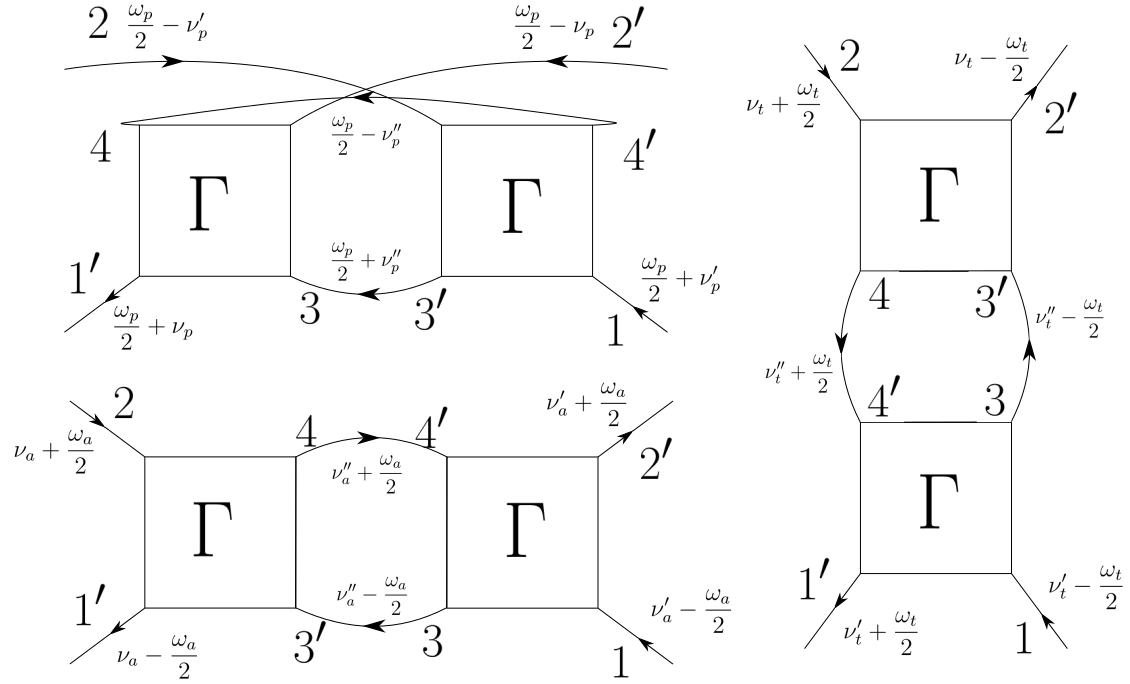
\includegraphics[width=\textwidth]{all-Bubbles.png}
	\caption{Bubbles in the respective channels}
\end{figure}




Thus, first of all, we have the frequency arguments that go into both propagators of  the bubble.  Now, as for the sole bubbles, their Keldysh structure gets simplified thanks to the causality constraint imposed by $G^{1|1}=0$. Thus, from the possible total of 16 Keldysh components, only 9 are not always zero and, if one chooses the following convention to define the indexation, these are the same for all channels, though the Keldysh structure of these elements not necessarily have to be the same. More precisely, the bubbles in the p-channel have a slightly different structure than the a- and t-channels that, due to their "conjugacy", take exactly the same structure.

For the a-channel, we have
\begin{align}
\Pi_a^{\alpha'_3\alpha'_4|\alpha_3\alpha_4} &= G^{\alpha'_3|\alpha_3}\left(\nu''_a-\frac{\omega_a}{2}\right)G^{\alpha'_4|\alpha_4}\left(\nu''_a+\frac{\omega_a}{2}\right)\\
\begin{pmatrix}
0  & 1  & 2   & 3\\
4  & 5  & 6   & 7\\
8  & 9  & 10 & 11\\
12& 13&14 & 15
\end{pmatrix} &=
\begin{pmatrix}
1111 & 1112 & 1121 & 1122 \\
1211 & 1212 & 1221 & 1222\\
2111 & 2112 & 2121 & 2122\\
2211& 2212 & 2221 & 2222
\end{pmatrix} = \begin{pmatrix}
0    & 0    & 0    & AA \\
0    & 0    & AR & AK\\
0    & RA & 0    & KA\\
RR & RK & KR & KK
\end{pmatrix},
\end{align}

for the p-channel
\begin{align}
\Pi_p^{\alpha'_3\alpha'_4|\alpha_3\alpha_4} &= G^{\alpha_3|\alpha'_3}\left(\frac{\omega_p}{2}+\nu''_p\right)G^{\alpha'_4|\alpha_4}\left(\frac{\omega_p}{2}-\nu''_p\right)\\
\begin{pmatrix}
0  & 1  & 2   & 3\\
4  & 5  & 6   & 7\\
8  & 9  & 10 & 11\\
12& 13&14 & 15
\end{pmatrix} &=
\begin{pmatrix}
1111 & 1112 & 1121 & 1122 \\
1211 & 1212 & 1221 & 1222\\
2111 & 2112 & 2121 & 2122\\
2211& 2212 & 2221 & 2222
\end{pmatrix} = \begin{pmatrix}
0    & 0    & 0    & AR \\
0    & 0    & AA & AK\\
0    & RR & 0    & KR\\
RA & RK & KA & KK
\end{pmatrix},
\end{align}

and, lastly, for the t-channel, the same as for the a-channel:
\begin{align}
\Pi_t^{\alpha'_3\alpha'_4|\alpha_3\alpha_4} &= G^{\alpha'_3|\alpha_3}\left(\nu''_t-\frac{\omega_t}{2}\right)G^{\alpha'_4|\alpha_4}\left(\nu''_t+\frac{\omega_t}{2}\right)\\
\begin{pmatrix}
0  & 1  & 2   & 3\\
4  & 5  & 6   & 7\\
8  & 9  & 10 & 11\\
12& 13&14 & 15
\end{pmatrix} &=
\begin{pmatrix}
1111 & 1112 & 1121 & 1122 \\
1211 & 1212 & 1221 & 1222\\
2111 & 2112 & 2121 & 2122\\
2211& 2212 & 2221 & 2222
\end{pmatrix} = \begin{pmatrix}
0    & 0    & 0    & AA \\
0    & 0    & AR & AK\\
0    & RA & 0    & KA\\
RR & RK & KR & KK
\end{pmatrix}.
\end{align}
This is a good point to point out that it's only the internal structure of the bubble the one that is the same for the a- and t-channels. The way the legs are connected and, consequently, the following functions, do defer between both (and, actually, all three) channels.
These aforementioned functions are a devise to exploit the zeros in the bubbles \textit{and}, simultaneously, the fact that one only needs to store $n_{K_i}$ Keldysh components per diagrammatic class. These are functions that then, based on the Keldysh index, $i_0$, of the left hand side of Eq. \ref{eq:derivativeOfgamma} (i.e. $i_0\in\{0,\dots, n_{K_i}\}$ and the Keldysh index, $i_2$, of the list of non zero entries of the bubbles (i.e. $i_2\in\{3, 6, 7, 9, 11, 12, 13, 14, 15\}$)  determine precisely the corresponding components $i_1$ and $i_3$ for the vertices left and right of the bubble in Eq. \ref{eq:derivativeOfgamma}. Condensed into an equation, the statement is as follows:

\begin{equation}
\dot{\gamma_r}^{i_0}(\omega_r, \nu_r, \nu'_r) = \sum_{i_2\in BK} \int d\nu''_r \Gamma^{i^r_1(i_0, i_2)}(\omega_r, \nu_r, \nu''_r)  \dot{\Pi}_r^{i_2}(\nu_1^r, \nu_2^r)  \Gamma^{i^r_3(i_0, i_2)}(\omega_r, \nu''_r, \nu'_r),
\label{eq:fullgammaDerivative}
\end{equation}
where we have emphasized that the frequencies that go into the bubbles depend on the channel, as depicted above, that the indices $i_1$ and $i_3$ are functions of the other two indices and the way these are determined are also channel-dependent and $BK = \{3, 6, 7, 9, 11, 12, 13, 14, 15\}$.
Writing down the exact form of these functions is a straight-forward task, which requires the conversion of $i_0$ and $i_2$ into indices in the $\{1111, \dots, 2222\}$ set. To visualize the process, just look at the figures drawn above. There, it becomes apparent, that, for $i_0 \rightarrow \alpha'_1\alpha'_2|\alpha_1\alpha_2$ and $i_2 \rightarrow \alpha'_3\alpha'_4|\alpha_3\alpha_4$, the functions are as follows:

\begin{align}
i_1^a (\alpha'_1\alpha'_2|\alpha_1\alpha_2, \alpha'_3\alpha'_4|\alpha_3\alpha_3) &= \alpha'_1\alpha_4| \alpha'_3\alpha_2 \\
i_3^a (\alpha'_1\alpha'_2|\alpha_1\alpha_2, \alpha'_3\alpha'_4|\alpha_3\alpha_3) &= \alpha_3\alpha'_2| \alpha_1\alpha'_4 \\
i_1^p (\alpha'_1\alpha'_2|\alpha_1\alpha_2, \alpha'_3\alpha'_4|\alpha_3\alpha_3) &= \alpha'_1\alpha'_2| \alpha'_3\alpha_4 \\
i_3^p (\alpha'_1\alpha'_2|\alpha_1\alpha_2, \alpha'_3\alpha'_4|\alpha_3\alpha_3) &= \alpha_3\alpha'_4| \alpha_1\alpha_2 \\
i_1^t (\alpha'_1\alpha'_2|\alpha_1\alpha_2, \alpha'_3\alpha'_4|\alpha_3\alpha_3) &= \alpha_4\alpha'_2| \alpha'_3\alpha_2 \\
i_3^t (\alpha'_1\alpha'_2|\alpha_1\alpha_2, \alpha'_3\alpha'_4|\alpha_3\alpha_3) &= \alpha'_1\alpha_3| \alpha_1\alpha'_4 \\
\end{align}
\subsection*{Structure of the internal bubble - diagrammatic classes' contributions}
Now, at this stage, the natural question to ask is how the \textit{diagrammatic} decomposition of Eq. \ref{eq:fullgammaDerivative} looks like i.e., given that $\dot{\gamma_r} = \sum_i \dot{K_r^i}$, what are the diagrammatic classes that contribute to each of these derivatives? It should by now be clear that not all classes can contribute to all derivatives, since, for instance, diagrams in the $K_3$ class, by definition, do not fulfill the requirement of having, say, two lines connected to the same vertex on one side. Thus, no terms with $K_3$ can appear in $\dot{K_1}$.
The natural thing to do at this stage is, basically, classify by sides and lines connected to one vertex, what classes fulfill the requirements to contribute, at least on one side, to which ones.
Thus, one can establish the following categorization:

\begin{center}
\begin{tabular}{| c| | c | c|} 
\hline
          &  L & R \\ 
          \hline\hline
 SV   & $K_1^r$, $\bar{K_2^r}$ &  $K_1^r$, $K_2^r$\\ 
  DV & $K_2^r$, $K_3^r$, $\gamma_{\bar{r}}$  & $\bar{K_2^r}$, $K_3^r$, $\gamma_{\bar{r}}$\\ 
 \hline
\end{tabular}
\end{center}
Here, SV and DV stand for ''same vertex'' and ''different vertex'', alluding to whether or not both lines to the right (R) of the left (L) of the vertex connect to the same or to different vertices. The inclusion already of $\gamma_{\bar{r}}$ is due to the foreshadowing of the multi-loop iterative loop i.e., we will be interested in feeding back diagrams of channels $\bar{r}$ to calculate higher loop order contributions to channel $r$.
Through this, one then gets the following Contribution Table to $\dot{K_i^r}$:

\begin{center}
\begin{tabular}{| c| | c | c|} 
\hline
          &  L & R \\ 
          \hline\hline
 $\dot{K_1^r}$  & $K_1^r$, $\bar{K_2^r}$&  $K_1^r$, $K_2^r$\\ 
 $\dot{K_2^r}$ & $K_2^r$, $K_3^r$, $\gamma_{\bar{r}}$  & $K_1^r$, $K_2^r$\\
 $\dot{\bar{K_2^r}}$ & $K_1^r$, $\bar{K_2^r}$ & $\bar{K_2^r}$, $K_3^r$, $\gamma_{\bar{r}}$\\ 
 $\dot{K_3^r}$ &  $K_2^r$, $K_3^r$, $\gamma_{\bar{r}}$   & $\bar{K_2^r}$, $K_3^r$, $\gamma_{\bar{r}}$\\
 \hline
\end{tabular}
\end{center}

What this table summarizes is the possible terms that can appear on the RHS of \ref{eq:derivativeOfgamma}, if one decomposes it into the diagrammatic classes.
















\end{document}
